\documentclass[11pt,letterpaper]{scrartcl}

\usepackage[english]{babel}
\usepackage[utf8x]{inputenc}
%\usepackage{amsmath}
\usepackage{graphicx}
%\usepackage[colorinlistoftodos]{todonotes}
\usepackage{comment}
\usepackage[T1]{fontenc}
\usepackage{authblk}
\usepackage{booktabs}
\usepackage[authoryear]{natbib}

\title{Discovering Cryptic Breeding Sites by Radio Tracking Coconut Rhinoceros Beetles, \textit{Oryctes rhinoceros} (Coleoptera: Scarabaeidae)}

\author[1]{Diego ?. Barahona}
\author[1]{Katherine A. Lehman}
\author[2]{Aubrey Moore}
\author[3]{Domenik ?. Skabeikis}
\author[2]{Ian R. Iriarte}
\author[3]{Eric B. Jang}
\author[1,*]{Matthew S. Siderhurst}
\affil[1]{Department of Chemistry, Eastern Mennonite University, 1200 Park Road, Harrisonburg, VA, 22802, USA}
\affil[2]{College of Natural and Applied Sciences, University of Guam, Mangilao, Guam 96923, USA}
\affil[3]{Daniel K. Inouye U.S. Pacific Basin Agricultural Research Center, Agricultural Research Service,
United States Department of Agricultural, 64 Nowelo St., Hilo, HI 96720, USA}
\affil[*]{Corresponding author: \texttt{matthew.siderhurst@emu.edu}}

\begin{document}
\maketitle
% * <aubreymoore2013@gmail.com> 2016-01-09T10:04:06.717Z:
%
% The Judas goat analogy may not be apparent to many readers. I suggest leaving this out.
%
% ^.
\begin{abstract}
Coconut rhinoceros beetle (CRB), \textit{Oryctes rhinoceros} L., is a serious pest of coconut trees and other palms throughout Southeast Asia and on  several Pacific Islands \citep{VanderMeer1987}.  Adults kill palms when they bore into crowns to feed on sap. Larvae feed only dead plant material at breeding sites. Eradication is possible if all breeding sites are located and destroyed. A field trial was performed on Guam to test the feasibility of using radio-tagged adults to discover cryptic breeding sites. Of 33 radio-tagged beetles that were released, 19 were successfully tracked to landing sites, X of which were considered to be active or potential breeding sites. The remaining 14 beetles were lost when they flew beyond the range of our receivers. None of the radio-tagged beetles were caught in numerous pheromone traps near release sites.
\end{abstract}
The coconut rhinoceros beetle (CRB), Oryctes rhinoceros L. (Coleoptera: Scarabaeidae, Dynastinae), is a serious pest of coconut trees, Cocos nucifera L., and other palms throughout the Pacific and Southeast Asia. CRB damage to coconut trees can result in a mortality rate of up to 50\% as reported in Palau in 1953 (Gressit 1953, Jackson 2010). Although CRB damage does not always result in coconut tree mortality, the characteristic V-cut damage to palm fronds can adversely affect the aesthetic value of ornamental trees, which is especially problematic in tourist areas. Such is the case in Guam, where unmanaged palms show CRB damage in close to 100\% of the palms near the highly touristic Tumon waterfront area (Moore, Jackson 2010). 

CRB damage to palms is caused almost exclusively by adult CRB feeding in coconut tree crowns, with larvae causing little or no economic damage as they feed on decaying plant material. Typically, adult beetles bore into the apical meristematic tissue of palm trees and feed on the base of unopened fronds, resulting in V-cuts once fronds open (Bedford 2013, Hinckley 1973). Once fed, adult CRB fly in search of breeding sites to mate. Adult CRB generally repeat this cycle of feeding and mating until they can no longer fly from feeding to breeding sites (Paper). This behavioral pattern is problematic for pest management efforts since CRB can breed in a wide range of locations, which tend to be difficult to find (Bedford 2013, Hinckley 1973). Sources in Malaysia and Guam have reported breeding sites in shredded palm trunk material, palm frond debris, compost heaps, and dead palm trunks, all of which are abundant in these tropical countries, and this high abundance of breeding sites leads to higher damage by CRB (Bedford 1976, Bedford 2013).

CRB monitoring and control utilizes a number of management techniques. These include biological control methods, which have played an essential role in the control of CRB populations. Biocontrol of CRB larvae mainly consists of using the fungal species Metarhezium anisopline, which has been reported to effectively control larvae populations (Arura 1984, Bedford 2013, Ferron et al. 1974). On the other hand, adult CRB biocontrol relies on the use of viral control agents. Infection with Baculovirus oryctes has successfully decreased CRB populations in various nations of Southeast Asia and the Pacific where infected individuals were released (Bedford 1985, Lomer 1985, Gorick 1980). However, recent studies report that the Guam CRB biotype has seemingly developed resistance to the viral control agent, creating an even more dire situation for the control of CRB (Moore, Jackson 2010). 

Traps and lures have also been employed in CRB monitoring and surveillance efforts. Bioassay studies have reported several lures that attract adult CRB. Of these lures, ethyl 4-methyloctanoate, the CRB aggregation pheromone, has had fairly good results (PAPER, Vander Meer 1979, Vander Meer 1983). However, traps utilizing this lure in Papua New Guinea have had moderate success with an average of 131 CRB caught per trap over a 19 week period (Bedford 1975). The situation is worse in Guam, where trap systems have not provided successful control of CRB, with catching rates as low as 0.0006 beetles per trap per day (Moore, Jackson 2010). 
Finding and destroying breeding sites has been an integral part of CRB eradication programs both in Guam and in Hawaii. However, the cryptic nature of CRB breeding sites makes them difficult to discover. Therefore, there is a pressing necessity to develop methods to reliably discover cryptic CRB breeding sites. Trained dogs have been utilized to detect pest insect locations with olfactory cues in several studies with moderate success (sources). However, the training of dogs is an expensive process and may have limited usefulness for discovering breeding sites in trees. Alternatively, predators/parasitoids or conspecifics of pest insects have evolved superior sensory systems to find either prey or mates in a complex natural environment and are the most adequate agents to detect a species. Following this idea, a novel way to detect pest insects in the wild has been recently discovered. Swink (et al.) described the use of the predatory wasp Cerceris fumipennis, a natural predator of different beetles in the Buprestidae family, to specifically monitor the emerald ash borer. Although this biological control agent succeeded in capturing a large number of beetles, C. fumipennis could not serve as a selective control agent as it collected samples of 52 different species in 11 different genera (Swink 2013). An obstacle to using conspecifics is the necessity to have the capability of following the marked individual. This problem is thoroughly addressed by using radio telemetry to investigate insect populations and behavior. Rink and Sinsch have utilized radio telemetry to study population migration and connectivity of the stag beetle Lucanus Cervus in order to define conservation efforts for the species (Rink and Sinsch 2007). Similarly, Beaudoin-Olliver (et al.) has implemented radio telemetry to successfully describe the flight behavior of the species Scapanes australis of the Dynastinae subfamily, to which CRB belongs (Beaudoin-Olliver 2003). In both of these cases, radio telemetry proved to be able to successfully track individual beetles, elucidating its potential use in the control of insect pests with conspecifics. 

The semio-chemical communication adult CRB utilize to find mates in breeding sites provide a prime opportunity to locate cryptic breeding sites. This chemical communication signaling can be exploited by using radio telemetry to follow adult CRB that are seeking these cryptic breeding sites. This study seeks to develop a control mechanism that uses laboratory-reared CRB equipped with miniature radio-tracking devices to identify cryptic breeding sites, which could then be treated, removed or destroyed. 

\section*{Materials and Methods}

\subsection*{Release sites and experimental conditions} 

Tagged CRB were radio tracked after release at two locations on Guam: Triton Farm University of Guam, Dededo (13°31'56.8"N 144°52'24.0"E) and Asan Beach National Park, Hagåtña (13°27'57.5"N 144°42'39.4"E). Triton Farm is an inland experimental farm bordered by a residential area and uncultivated forest areas that include coconut palms along with other trees. Asan Beach National Park is roughly triangular with the ocean bordering one side, coastal wetlands on another, and forested hillside on the third. The park itself is a large, open, grassy field and includes with coconut palms on the edges, many of which displayed CRB damage at the time of the study. Thus, both sites feature relatively accessible terrain that provides a variety of potential breeding sites as well as adult food sources. At each study location, a grassy, open area was chosen for CRB release.

Weather conditions during the experiment were mainly clear with occasional periods of rain and overcast skies. On release dates, August 8 to August 14, average temperature ranged from 27°C to 29°C while relative humidity was 80\% to 88\%. Beetles were generally tracked under clear skies with the exception of August 9 during which light showers occurred. 

\subsection*{Oryctes rhinoceros capture and specimen selection}

CRB used for radio tracking were wild-caught in bucket traps containing oryctalure and collected within one week of capture. These beetles were placed in tubs containing moist peat moss, fed fresh banana slices and allowed to rest for at least three days.

Only CRB capable of flight were selected for radio tagging and release. After the rest period, captured beetles were flight tested at least one day prior to experimentation. The flight test chamber consisted of a large 121 L lidded garbage container. Within the chamber, about 30 beetles were placed in a smaller open metal bowl half filled with moist peat moss atop an upside down 19 L bucket. Beetles could only exit the smaller open container by flying out of it; therefore, any beetle found on the bottom of the flight chamber container the next morning was considered flight-capable. Flight capable CRB were transported and stored until release in lidded plastic bins approximately 45 cm by 30 cm by 18 cm containing 4 to 6 inches of damp peat moss. Because not all beetles flew when first taken into the field, some beetles remained in storage for up to six days.

\subsection*{CRB preparation}

Beetles that demonstrated flight capacity were marked with a unique four-digit code engraved on one elytrum using a laser engraver (Fenix Flyer, Synrad Inc., Mukilteo, WA, United States). The sex, mass and elytral dimensions of each beetle were then recorded. Both male and female specimens were used.

Prior to transmitter attachment, the beetle pronotum was abraded with sandpaper to improve adhesion. Transmitters were then affixed to the pronotum with hot melt glue (product xxxx company location xxx model number xxx)(Figure XX picture?) and steady pressure was applied as the adhesive hardened. Each glue-on transmitter (model A2414; Advanced Telemetry Systems; Isanti, Minnesota) had a mass of approximately 300 mg and was secured with approximately 250 mg of adhesive.

\subsection*{Tracking equipment}

Transmitters had a maximum battery life of 45 days with a warranty guarantee of 22 days. Two frequency bands were chosen ranging from 148.641 to 148.992 and 164.032 to 164.409. Frequencies used with individual CRB were recorded in conjunction with beetle identification numbers. 

Beetles were tracked using a radio receiver (model R410, Advanced Telemetry Systems, Isanti, Minnesota) equipped with a three-element folding Yagi antenna (model 13863, Advanced Telemetry Systems, Isanti, Minnesota) attached to a. A total of four units were used so that multiple beetles could be tracked simultaneously: two receivers were programmed with bandwidths from 148.641 to 148.992 and two with bandwidths 164.032 to 164.409. In addition to radio tracking equipment, handheld GPS units (model XXX, Garmin, XXX) were used to record locations where beetles were found or point of signal loss for each beetle. 

\subsection*{Beetle release and tracking procedure}

Beetles were transported to release sites in plastic storage bins. The lid of the bin was removed at dusk (roughly 19:30) and the container was closed at roughly 21:30. Once the containers were opened, CRB activity was carefully monitored using an infrared camera. Observation under the infrared camera revealed that beetles thermal profile would change just prior to flight, and thermally active beetles observed emerging from the peat moss were briefly viewed under red light to record the identification number and determine the frequency of the radio transmitter. Though nearly all beetles flew independently, several beetles that had not yet flown by the end of experimentation were encouraged to flight by removing them from the peat moss and throwing them into the air to facilitate takeoff.

CRB were pursued on foot following release and were tracked until a landing site was determined or until the transmitter signal was lost. In either case, a waypoint was recorded at the landing site or the last point of signal reception using a GPS unit.

Landing sites were visited on the following morning, and attempts were made to more precisely determine the location of each beetle. Beetle locations were monitored over several days, and beetles and or transmitters were recovered when possible at the end of the experiment.  CRB and transmitters were successfully recovered by digging up beetles that buried into soil or compost; however the locations of CRB tracked to coconut crowns could not be as exactly determined due to the density of the frond foliage. 

\subsection*{Analysis}

In assessing the flight patterns of beetles for trends between sex and size, percent emergence weight (\%EW) was calculated as an additional consideration. Percent emergence weight describes CRB mass at the time of measurement relative to its estimated mass upon emergence. This value can be estimated based upon a linear equation relating elytral measurements and emergence weight (Vander Meer and Mclean, 1975). This value is significant in data analysis because \%EW reflects the present life stage of a beetle and how much stored energy it has available; CRB emerge at their heaviest weight and gradually lose weight over their lifespan.  

-GIS (Diego)

-stats (Matt)

\section*{Results}

The tagging and radio tracking of CRB in this study led to the successful location of multiple cryptic breeding sites at both experiment sites. CRB were most active from approximately 19:30 to 21:00, and flight activity did not appear to be heavily influenced by the prevailing weather conditions. Transmitters did not inhibit the flight mechanics of CRB to an observable degree. Over the course of experimentation, it was observed that beetles employed thermogenesis in flight muscles directly prior to flight, allowing a reliable prediction to be made as to which beetles were about to fly by detecting thermal radiation with an infrared camera. 

	A total of 33 out of 34 beetles tagged for release flew during the course of this study. Of the 33 beetles that flew, 19 were successfully tracked to landing sites (Figure 1). The \% EW for CRB that were successfully located, 78 ± 2\%, and for CRB that were lost, 72 ± 2\%, differed significantly (t-test: P = 0.021).  However, EW (P = 0.822) and weight (P = 0.510) did not differ between CRB that were successfully tracked or lost after release.  Additionally, there were no differences in the numbers of male and female CRB that were successfully located or lost (Fisher’s: P = 1.000). 
    
No relationship was found between the distance beetles moved from the release point and beetle EW (R2 = 0.0686), \%EW (R2 = 0.0462), or weight (R2 = 0.0465).  There was no difference in the mean distance beetles moved at the two experimental sites, Yigo, 276 ± 42 m, and Asan, 215 ± 57 m (P = 0.408).  Additionally, no differences were found between the mean distances male (254 ± 44 m) and female (233 ± 61 m) beetles moved (P = 0.778).  

Landing locations of CRB were categorized by microhabitats described as other trees, coconut crown, traps, base of trees, or soil unassociated with trees or traps. Percent emergence weight varied significantly by the microhabitat to which CRB were tracked (Figure 2a., ANOVA: F = X.XXX, P = X.XXX). Microhabitats of CRB were further clustered as arboreal (> 1 m above ground) or terrestrial destinations (< 1 m above ground) (Figure 2b.).  When microhabitats were grouped as either arboreal or soil-associated, the difference in mean \%EW between the groups, arboreal, 74 ± 2\%, soil-associated, 82 ± 3\%, was found to be highly significant (t-test: P < 0.001).   In addition, while emergence weight (EW) was significantly different between arboreal (6.5 ± 0.4 g) and soil-associated (4.9 ± 0.5 g) microhabitats (t-test: P = 0.020), there were no differences in weight (P = 0.160) or distance travelled (P = 0.908) between these microhabitat groupings.  The numbers of male and female beetles did not vary between arboreal and soil-associated microhabitats (Fisher’s: P = 1.000).

Arboreal destinations were most commonly the crowns of coconut palms damaged by bore holes; however, beetles also landed in the branches of other species of trees. For example, an upper branch of a large breadfruit tree damaged in a recent typhoon was the final destination of one beetle. Upon investigation, several other beetles and grubs were found in the rotting limb along with the radio transmitter. In another instance, two beetles flew to the crown of the same highly damaged coconut tree independently of one another. 

In soil associated landing site, CRB tended to bury into the soil upon landing at depths up to approximately 15 centimeters. Typically, these sites were at the base of a tree. Four out of five of these landing sites were at the base of coconut palms, though CRB also landed in less predictable locations. For example, one beetle landed beneath a trailer parked on a grassy lawn in a residential area surrounding Triton Farm. In another example of particular interest, one beetles was found beneath a CRB barrel trap baited with oryctalure at each experiment site. Other beetles and larvae were found also beneath one of these traps. 

\section*{Discussion}

This study was successful in tracking CRB to cryptic breeding sites at two locations on the island of Guam.  The two areas where CRB were tracked differed both in topography and vegetation and the effective location of tagged beetles in these different environments shows promise for the applicability of this technique in the varied habitats were CRB infestations may occur. Out of 33 released CRB, a total of 19 were retrieved either as an individual or as a fallen radio transmitter resulting in a 58\% retrieval rate. This comparatively high retrieval rate required an input of approximately 1 hour per CRB immediately after release and at least the same amount of time on the following day. The tracking of CRB to an approximate location during the night followed by a more precise pinpointing during the daytime proved to greatly facilitate the retrieval of released CRB.

\section*{ANECTDOTAL LOCATIONS}

Although a majority of the released CRB were successfully tracked to discrete locations, 14 CRB were lost presumably due to out-of-range flights. Interestingly, those CRB that flew out of range had statistically significantly lower percent emergence weights than those that stayed within the detection range of the radio devices, suggesting that lighter CRB fly longer distances. State average \%EW. Although the distance flown by retrieved CRB had no statistically significant correlations with percent emergence weight, distance flown by all 33 CRB, lost and found, would most likely correlate with percent emergence weight if the distance of the lost CRB were to be determined. This observation raises the ability to minimize the loss of CRB while radio tracking. Prior to release, CRB must be fed to above 70 percent of their emergence weight to ensure that the individuals will remain within the detection radius. 

Moreover, percent emergence weight of released CRB had a strong association with the microhabitats in which tagged CRB were found. Of the 19 retrieved CRB, 11 landed arboreal microhabitats whereas 8 landed in soil-associated microhabitats. The CRB that landed in the arboreal microhabitats had a statistically significantly lower percent emergence weight than those CRB that landed on soil-associated microhabitats, 74.43\% compared to 82.73\% respectively. It has been noted that adult CRB spend their time either feeding on the crown of palms or breeding in either soil or compost piles (Zelazny 1975). As CRB alternate between these microhabitats, individuals fluctuate in their percent emergence weight making it possible to determine the behavioral pattern that CRB will engage in by noting their percent emergence weight (Source).  CRB at a higher percentage of their emergence weight will very likely refrain from further feeding and fly in search of breeding sites whereas CRB at a lower percentage of their emergence weight will likely forage in search for food. Therefore, it is not coincidental that the CRB that landed in ground microhabitats, associated with breeding, had statistically significantly higher percentage emergence weights than those that landed in palm crowns, associated with feeding sites. This characteristic of the CRB life cycle makes this tracking method specific and controllable. In order to have CRB fly directly to breeding sites, the individuals must be fed to above 80 percent of their emergence weight. In doing so, monitoring and eradication teams can ensure that the released CRB will not lead them to feeding sites rather than breeding sites and will increase the effectiveness of CRB control methods. It is reasonable to hypothesize that heavier CRB landed on lower microhabitats due to the comparative inability to reach higher altitudes than the ones reached by lighter CRB. However, all of the released CRB flew several meters vertically into the air before displacing horizontally. If heavier CRB experienced a hindered vertical displacement in comparison to lighter CRB, then takeoff would have notably different between these two groups. Since hindered vertical displacement was not observed during CRB takeoff, it is reasonable to conclude that the difference in landing microhabitats was most likely due to the percent emergence weight of released CRB. 

The use of radio telemetry to monitor flying species is generally constrained by the weight of radio transmitters (Robinson et al. 2009, Cochran et al. 2004, Thorup et al. 2007). This limitation is especially true when monitoring flying insects since a small increase in weight may severely hinder flight behavior (Source). In recent years, though, the gradual miniaturization of transmitters has circumvented this obstacle allowing for more precise monitoring of flying insects (Sato Maharbiz 2010). One of the factors determining the feasibility of this study was whether or not adult CRB could fly undisturbedly with the attached radio transmitters. Adult CRB are excellent fliers and can exert force much larger than their body weight when fighting and boring, so it was reasonable to expect that the miniature radio transmitters would have little to no effect on CRB flight capability. As expected, the flight capability of CRB was seemingly unaffected by the extra weight of radio transmitters.  Each radio transmitter amounted to between 5.04\% and 9.72\% of the CRB weight at the time of release, and there was no correlation between the increased percentage weight and the single flight distance of CRB indicating that CRB could fly carry the extra burden of the radio transmitters. Note about whether it went over 100\% It is also important to note that the 14 CRB were lost did present not statistically significant differences in the radio transmitter percentage weights compared to the CRB that stayed in range. These observations are consistent with other studies monitoring members of the Scarabaeidae family which found that radio transmitters did not noticeably affect beetle flight capabilities (Beaudoin-Ollivier 2003, McCollough 2006, Rink and Sinsch 2007). Also, the duration of commercially available radio transmitters (10-14 days) is appropriate for this type of CRB monitoring. However, the battery life of the transmitters must guide monitoring protocol timelines. CRB should be pinpointed to a final location within 2-3 days after initial release to prevent the loss of CRB due to battery drainage. 

Another important factor to consider is the distance over which CRB can be monitored. Radio telemetry monitoring typically covers only short to medium displacement distances usually limiting the applications of the technology (Robinson et al.2009). The radio devices employed in this study had an effective range of localization that varied with topological conditions. In this study, the range of detection was appropriate for monitoring since the overall CRB flight distance from release sites to landing sites ranged from 52.8 meters to 564.6 meters. This range also roughly delineates a radius for breeding site discovery from released CRB; the detector CRB must be released no further than approximately 500 meters from breeding sites. This might present difficulties for eradication teams since the breeding sites in question occur in cryptic locations presumably unknown to those searching for them. The relatively short detection radius of the radio devices obligates teams to close in on the cryptic sites through other investigative means. In order to effectively estimate possible locations of CRB breeding site, visual monitoring of damage and trapping should assess the presence of CRB populations. Once visual monitoring and trapping indicates the existence of CRB in a particular location, the detector CRB would be released in the vicinity to pinpoint the exact location of the breeding sites. Stats about monitoring and visual in Guam and HI This combination of monitoring methods would ease the control and eradication of CRB, and since traps and visual monitoring are already widespread, it would not be complicated to craft an integrated strategic plan. 

\section*{COMPARATIVE TO OTHER METHODS}

\bibliographystyle{plainnat}
\bibliography{references}

\begin{figure}[p]
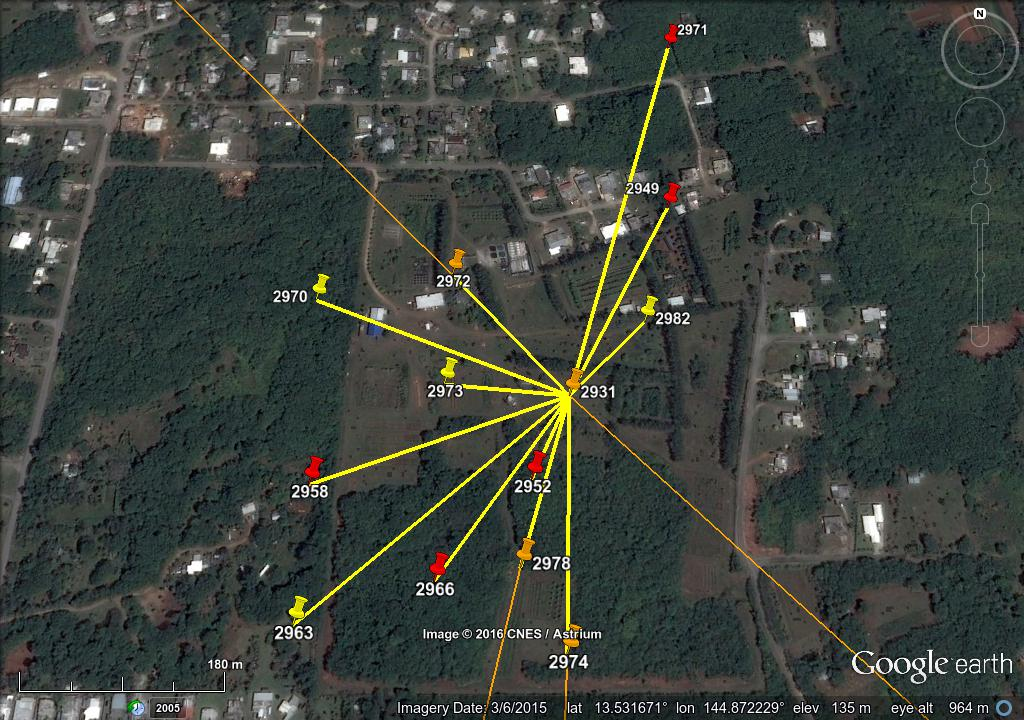
\includegraphics[width=\textwidth]{yigo_tracks.jpg}
\caption{\label{fig:yigo_tracks}Caption needed here.}
\end{figure}

\begin{figure}[p]
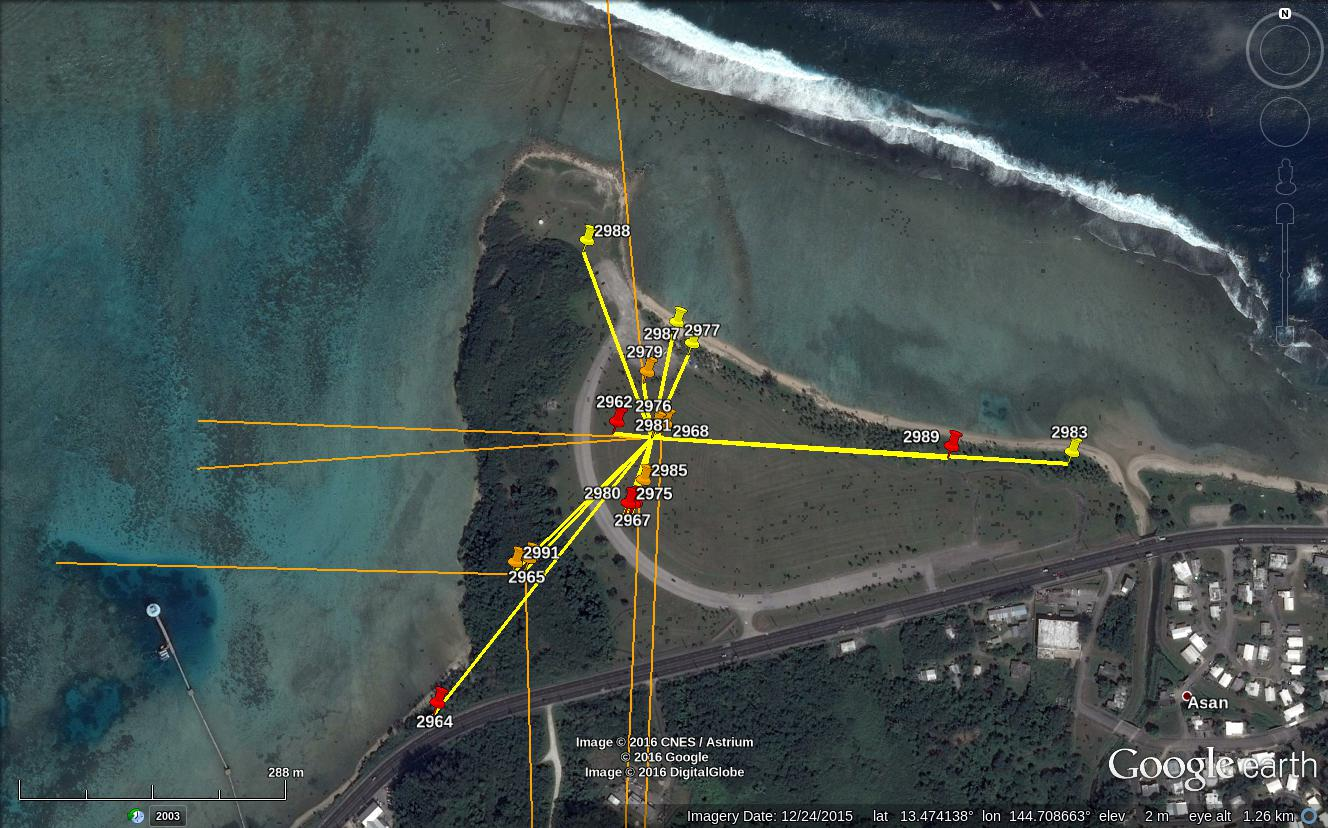
\includegraphics[width=\textwidth]{asan_tracks.jpg}
\caption{\label{fig:asan_tracks}Caption needed here.}
\end{figure}

\begin{figure}[p]
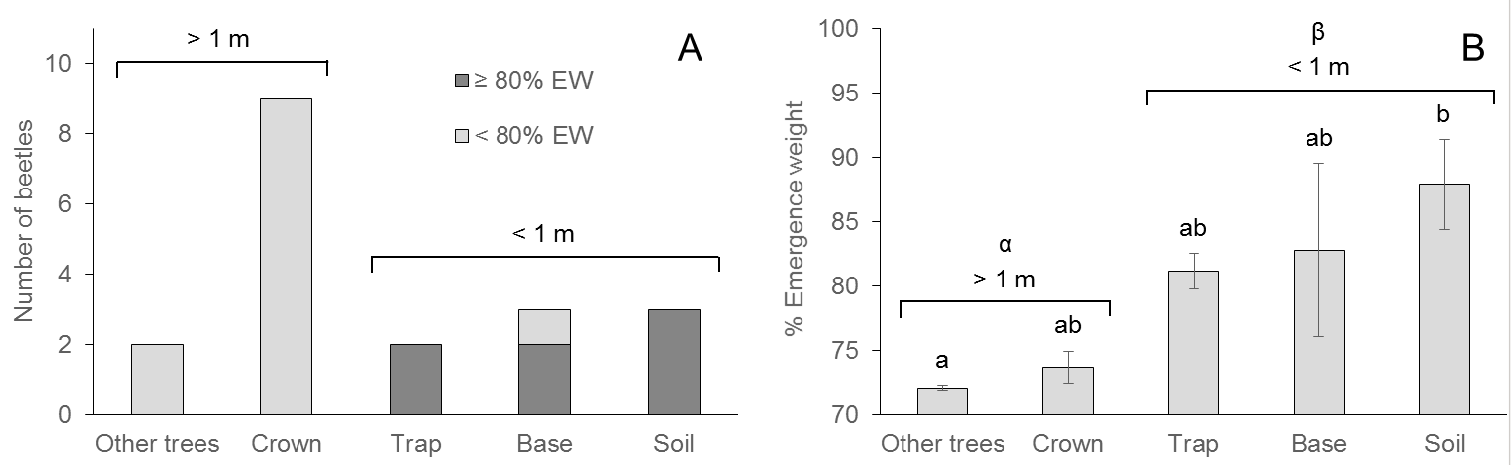
\includegraphics[width=\textwidth]{statsfig.png}
\caption{\label{fig:statsfig}Radio tracked coconut rhinoceros beetles grouped by microhabitat of discovery location. (A) Numbers of beetles tracked to different microhabitats including an indication of percent emergence weight.  (B) Percentage emergence weight of beetles (mean ± SE) grouped by microhabitat.  Lower case letters represent significant differences (p < 0.05) between beetles found in different microhabitats (Tukey’s HSD).  Greek letters represent significant differences between beetles tracked to arboreal microhabitats (> 1 m above ground) or soil-associated microhabitats (< 1 m above ground) (t-test, p < 0.001).}
\end{figure}

\begin{table}[p]
\begin{tabular}{lrrllrrlrlllllrrr}
\toprule
{} &  beetle\_id &  frequency & rel\_site &                                                                                  Notes &       lat2 &        lon2 &                   t2 &  extended\_track\_bearing & end\_point\_located & in\_tree & breeding\_site & flight\_test\_date & Sex &  Length &  Width &  Weight \\
\midrule
0  &       2968 &    148.641 &     Asan &                             weak signal coming from swamp across from Asan Park; swamp &  13.473933 &  144.708633 &     2015-08-11 09:18 &                  180.00 &             False &     NaN &           NaN &       2015-08-10 &   f &   21.17 &  16.47 &   2.641 \\
1  &       2977 &    148.671 &     Asan &                                             Found at base of coco tree; just off beach &  13.474933 &  144.708750 &           2015-08-11 &                     NaN &              True &   False &           NaN &       2015-08-10 &   f &   21.83 &  16.99 &   3.622 \\
2  &       2991 &    148.693 &     Asan &                                                                    Lost west over hill &  13.472575 &  144.707141 &  2015-08-12 19:58:50 &                  270.00 &             False &     NaN &           NaN &       2015-08-11 &   m &   25.86 &  20.63 &   5.774 \\
3  &       2981 &    148.703 &     Asan &                                                          Lost west over hill; no track &        NaN &         NaN &                  NaN &                  270.00 &             False &     NaN &           NaN &       2015-08-10 &   f &   24.94 &  18.96 &   5.206 \\
4  &       2971 &    148.732 &     Yigo &                                                         top of coconut tree adjust GPS &  13.535104 &  144.873882 &     2015-08-12 11:00 &                     NaN &              True &    True &           NaN &       2015-08-10 &   m &   22.36 &  17.55 &   3.087 \\
5  &       2929 &    148.752 &      NaN &                                                                         lost; no track &        NaN &         NaN &           2015-08-10 &                     NaN &             False &     NaN &           NaN &       2015-08-05 &   f &   25.41 &  20.29 &   4.220 \\
6  &       2985 &    148.764 &     Asan &                                                             out of range; towards road &  13.473374 &  144.708416 &     2015-08-10 21:01 &                  180.00 &             False &     NaN &           NaN &       2015-08-10 &   f &   22.80 &  18.07 &   4.017 \\
7  &       2963 &    148.782 &     Yigo &                                                    under trailer in the dirt; no track &  13.529393 &  144.870394 &     2015-08-12 12:36 &                     NaN &              True &   False &           NaN &       2015-08-10 &   m &   20.33 &  16.28 &   3.179 \\
8  &       2952 &    148.792 &     Yigo &                                               beetle in breadfruit tree; 2952?; wooded &  13.530583 &  144.872400 &     2015-08-10 09:30 &                     NaN &              True &    True &          True &       2015-08-05 &   f &   24.07 &  18.67 &   4.229 \\
9  &       2978 &    148.820 &     Yigo &                                                        faint signal in woods; no track &  13.529850 &  144.872300 &     2015-08-11 20:58 &                  196.44 &             False &     NaN &           NaN &       2015-08-10 &   m &   25.22 &  20.15 &   5.213 \\
10 &       2982 &    148.851 &     Yigo &                                              under barrel \#12, saw beetle, left beetle &  13.532033 &  144.873467 &     2015-08-12 09:18 &                     NaN &              True &   False &           NaN &       2015-08-10 &   m &   23.47 &  18.75 &   4.672 \\
11 &       2987 &    148.873 &     Asan &                                                                        base of coconut &  13.474723 &  144.708906 &           2015-08-13 &                     NaN &              True &   False &           NaN &       2015-08-11 &   f &   23.31 &  18.31 &   3.758 \\
12 &       2970 &    148.873 &     Yigo &  found beetle in soil, transmitter \textasciitilde20 cm away, retrieved beetle; transmitter reused?? &  13.532250 &  144.870383 &     2015-08-12 10:00 &                     NaN &              True &   False &           NaN &       2015-08-10 &   m &   21.60 &  17.02 &   3.411 \\
13 &       2931 &    148.902 &     Yigo &                                        out of range, toward highschool? East; no track &        NaN &         NaN &           2015-08-10 &                  135.00 &             False &     NaN &           NaN &       2015-08-05 &   m &   24.36 &  18.60 &   4.367 \\
14 &       2958 &    148.932 &     Yigo &                                             in coconut tree with 6+ bore holes; wooded &  13.530546 &  144.870442 &     2015-08-11 11:00 &                     NaN &              True &    True &           NaN &       2015-08-05 &   f &   25.76 &  19.16 &   5.009 \\
15 &       2974 &    148.963 &     Yigo &                                         edge of dense woods, up high; wooded; no track &  13.529167 &  144.872683 &     2015-08-11 19:31 &                  181.72 &             False &     NaN &           NaN &       2015-08-10 &   m &   22.59 &  17.97 &   3.562 \\
16 &       2976 &    148.972 &     Asan &                                            Damaged wing, lost west over hill; no track &        NaN &         NaN &                  NaN &                  270.00 &             False &     NaN &           NaN &       2015-08-10 &   m &   23.63 &  18.40 &   3.803 \\
17 &       2962 &    148.992 &     Asan &                                                                            Coconut top &  13.473946 &  144.708144 &           2015-06-13 &                     NaN &              True &    True &           NaN &       2015-08-10 &   m &   26.73 &  21.19 &   6.041 \\
18 &       2980 &    164.032 &     Asan &                                                             in damaged coco tree crown &  13.473150 &  144.708310 &     2015-08-11 08:56 &                     NaN &              True &    True &           NaN &       2015-08-10 &   m &   25.96 &  20.97 &   5.951 \\
19 &       2989 &    164.058 &     Asan &                                                               Same place in coco crown &  13.473707 &  144.711533 &                  NaN &                     NaN &              True &    True &           NaN &       2015-08-11 &   m &   24.97 &  19.96 &   5.329 \\
20 &       2951 &    164.082 &      NaN &                                                      Lost east; no coordnates recorded &        NaN &         NaN &                  NaN &                   90.00 &             False &     NaN &           NaN &       2015-08-05 &   f &   24.90 &  19.14 &   5.025 \\
21 &       2967 &    164.107 &     Asan &                                                             in damaged coco tree crown &  13.473160 &  144.708330 &     2015-08-11 08:54 &                     NaN &              True &    True &           NaN &       2015-08-10 &   f &   23.40 &  18.15 &   4.208 \\
22 &       2972 &    164.132 &     Yigo &                                                                  lost into dense brush &  13.532510 &  144.871660 &     2015-08-12 11:07 &                  318.00 &             False &     NaN &           NaN &       2015-08-10 &   f &   25.31 &  19.82 &   4.433 \\
23 &       2964 &    164.157 &     Asan &                           on top of large coco tree on beach across the hill Asan Park &  13.471210 &  144.706360 &           2015-08-11 &                     NaN &              True &    True &           NaN &       2015-08-10 &   f &   24.03 &  18.71 &   4.211 \\
24 &       2988 &    164.182 &     Asan &                                            Found beetl under barrel trap. breedin site &  13.475751 &  144.707832 &                  NaN &                     NaN &              True &   False &          True &       2015-08-11 &   f &   26.41 &  21.01 &   6.439 \\
25 &       2949 &    164.208 &     Yigo &                                        in heavily damaged coco tree over fence; wooded &  13.533230 &  144.873760 &     2015-08-12 09:00 &                     NaN &              True &    True &           NaN &       2015-08-05 &   m &   26.15 &  20.90 &   5.942 \\
26 &       2979 &    164.232 &     Asan &                                       Lost at indicated coordinates; went out of range &  13.474440 &  144.708450 &           2015-08-10 &                  351.03 &             False &     NaN &           NaN &       2015-08-10 &   m &   24.31 &  19.01 &   4.563 \\
27 &       2983 &    164.258 &     Asan &                                                   In or around base of small coco tree &  13.473650 &  144.712750 &     2015-08-11 09:07 &                     NaN &              True &   False &           NaN &       2015-08-10 &   f &   22.07 &  17.35 &   4.126 \\
28 &       2975 &    164.282 &     Asan &                                                                On top of big coco tree &  13.473145 &  144.708264 &                  NaN &                     NaN &              True &    True &           NaN &       2015-08-10 &   m &   23.82 &  18.39 &   3.910 \\
29 &       2969 &    164.307 &      NaN &                                                                                    NaN &        NaN &         NaN &                  NaN &                     NaN &             False &     NaN &           NaN &       2015-08-10 &   f &   24.19 &  19.10 &   4.811 \\
30 &       2966 &    164.333 &     Yigo &                                         In coco tree crown in private property; wooded &  13.529730 &  144.871570 &     2015-08-12 11:43 &                     NaN &              True &    True &           NaN &       2015-08-10 &   f &   24.01 &  18.94 &   4.379 \\
31 &       2965 &    164.357 &     Asan &                                                        towards tall grass only up high &  13.472615 &  144.707277 &     2015-08-13 11:20 &                  180.00 &             False &     NaN &           NaN &       2015-08-10 &   f &   22.13 &  17.13 &   2.989 \\
32 &       2944 &    164.382 &     Asan &                                                                      Asan; Did not fly &        NaN &         NaN &                  NaN &                     NaN &               NaN &     NaN &           NaN &       2015-08-05 &   m &   22.93 &  17.73 &   2.881 \\
33 &       2973 &    164.409 &     Yigo &                                        in brush line around base of small papy; wooded &  13.531440 &  144.871610 &     2015-08-11 20:32 &                     NaN &              True &   False &           NaN &       2015-08-10 &   m &   21.25 &  16.50 &   3.289 \\
\bottomrule
\end{tabular}

\end{table}

\end{document}